\documentclass[10pt]{article}

% ===================== Packages =====================
\usepackage[margin=0.85in]{geometry}
\usepackage{graphicx}
\usepackage{float}
\usepackage{capt-of}
\usepackage{booktabs}
\usepackage{array}
\usepackage{multirow}
\usepackage{caption}
\usepackage{xcolor}
\usepackage{enumitem}
\usepackage{hyperref}
\usepackage{amsmath}
\setlist{nosep, itemsep=2pt, topsep=2pt, leftmargin=1.4em}


\title{\vspace{-1.5em}Assignment 1: Fine-Tune, Sanitize, Extract\\
\large COL873 - Trustworthy Large Language Models}
\author{Laksh Goel \\ 2023CS10848}
\date{}

\begin{document}
\maketitle
\vspace{-2em}

\noindent\textbf{Adapter weights:} \href{https://drive.google.com/drive/folders/12jnfl4Zaum3CU9o4sL7jN7CmvDe209c2?usp=drive_link}{Google Drive folder}.
\texttt{PartA/} holds the six sweep adapters A1--A6 (zipped); \texttt{PartB/} holds \texttt{best\_sanitizer} (a copy of A6). The A5 adapter used for the LoRA-vs-QLoRA comparison in Part B is in \texttt{PartA/}.

% =====================================================
\section{Part A}

\subsection{Setup}
\begin{itemize}
  \item Base model: \texttt{Qwen/Qwen2.5-1.5B-Instruct}; task: map \texttt{source\_text} $\to$ \texttt{target\_text}, loss masked to completion tokens only.
  \item Data: \texttt{data/partA\_train.jsonl} (20{,}000), \texttt{data/partA\_validation.jsonl} (2{,}000), used in full and unmodified.
  \item Common hyperparameters across all six runs: 2 epochs; LR $2\times10^{-4}$, cosine schedule, 3\% warmup; effective batch size 16 (per-device batch 16 $\times$ grad.\ accum.\ 1); seed 42.
\end{itemize}

\subsection{Sweep Results}

\begin{table}[H]
\centering
\caption{Part A sweep (from \texttt{results/partA\_sweep.csv}). Val F1 was computed with an earlier, buggy span-recovery step and is too low; see Section B.1. Bold: best in each column (lowest cost, loss and leak rate; highest throughput and F1).}
\label{tab:partA-sweep}
\resizebox{\textwidth}{!}{%
\begin{tabular}{@{}l l l c c c c c c c c c c@{}}
\toprule
Run & Method & Target modules & $r$ & $\alpha$ & Quant & Train. \% & Peak GPU (GB) & Wall-clock (s) & Tok/s & Val loss & Val F1 & Leak rate \\
\midrule
A1 & LoRA  & q,v                          & 8  & 16 & none & \textbf{0.071} & \textbf{29.06} & \textbf{2017.6} & \textbf{9720} & 0.0176 & 0.7683 & 0.0417 \\
A2 & LoRA  & q,k,v,o                      & 8  & 16 & none & 0.141 & 29.07 & 2213.5 & 8860  & 0.0133 & 0.7876 & 0.0384 \\
A3 & LoRA  & attn + gate,up,down          & 8  & 16 & none & 0.595 & 29.16 & 3492.1 & 5616  & 0.0099 & 0.8057 & 0.0388 \\
A4 & LoRA  & attn + gate,up,down          & 32 & 16 & none & 2.336 & 29.50 & 3607.3 & 5436  & 0.0099 & 0.8077 & 0.0379 \\
A5 & LoRA  & attn + gate,up,down          & 32 & 64 & none & 2.336 & 29.50 & 3589.9 & 5463  & \textbf{0.0094} & 0.8074 & 0.0383 \\
A6 & QLoRA & attn + gate,up,down          & 32 & 64 & 4bit & 3.990$^\dagger$ & 29.19 & 5487.4 & 3574  & 0.0098 & \textbf{0.8146} & \textbf{0.0372} \\
\bottomrule
\end{tabular}%
}
\\[2pt]{\footnotesize $^\dagger$A6 has the same 36.93M trainable parameters as A4/A5; the percentage is higher only because \texttt{bitsandbytes} stores 4-bit weights packed, so the reported total drops from 1.58B to 0.93B.}
\end{table}

\begin{figure}[H]
\centering
\includegraphics[width=0.8\textwidth]{results/partA_fig.png}
\caption{Left: validation entity F1 vs.\ trainable parameter fraction (log scale). Right: peak GPU memory vs.\ validation F1. A4 and A5 overlap in both panels. A6's x-position is shifted right by 4-bit weight packing (see Table~\ref{tab:partA-sweep}).}
\label{fig:partA}
\end{figure}

\subsection{Analysis}
\begin{itemize}
  \item \textbf{Which axis gives the most F1 for the cost.} Adding the other attention layers (A1$\to$A2) is the best deal: it doubles trainable parameters (0.07\%$\to$0.14\%), adds only 196\,s of training, and gains +0.020 F1. Adding the MLP layers (A2$\to$A3) gains a similar amount (+0.018) but costs 4.2$\times$ the parameters and 21 more minutes, because MLP matrices are much larger. Raising the rank (A3$\to$A4) or $\alpha$ (A4$\to$A5) is the worst deal: about 4$\times$ the parameters for no real change in F1 ($+$0.002 and $-$0.0003). Peak memory is almost the same for all runs (29.1--29.5\,GB), so memory does not separate them.
  \item \textbf{Where the curve flattens.} At A3. After that, a larger rank or $\alpha$ does not improve F1 (0.806, 0.808, 0.807). Validation loss still improves a little up to A5, so the F1 metric saturates earlier than the loss does.
  \item \textbf{QLoRA.} A6 is A5 with the base model in 4 bits. Accuracy did not drop: F1 went from 0.807 to 0.815 and leak rate from 0.038 to 0.037. It saved only 0.3\,GB of memory (about 1\%), because most memory goes to activations, not to the base weights. It was much slower: 35\% fewer tokens per second and 53\% longer training. For a 1.5B model QLoRA is not worth it; it helps only when the base model itself does not fit in memory.
\end{itemize}

% =====================================================
\section{Part B}

\subsection{Setup}
\begin{itemize}
  \item \textbf{Sanitizer: A6.} It has the highest validation F1 and the lowest validation leak rate of all six runs. It was trained on a 4-bit base, so it is also evaluated on a 4-bit base. We also evaluate \textbf{A5} (same settings, no 4-bit) to see the effect of 4-bit training alone.
  \item \textbf{Generation.} Greedy decoding with the same system prompt as Part A. The output is allowed up to the input length plus 32 tokens.
  \item \textbf{Test set.} All 2{,}000 rows of \texttt{partB\_test.jsonl} (12{,}779 PII spans, 27 labels).
\end{itemize}

\subsection{B.1 Span Recovery}
The model outputs text, not spans. We line up the input and the output with \texttt{difflib}, and each part of the input that was replaced by a \texttt{[LABEL]} tag becomes a predicted span with that label.

\textbf{Rules.} (1) Each tag is first replaced by one special character that never occurs in the data, so a tag is always one unit. (2) A 1--2 character letter/digit match between input and output is treated as a coincidence; short space/punctuation matches are kept as separators between spans. (3) A replaced input region containing a tag becomes one span labelled by its first tag; text changed without a tag is not a span but counts as over-masking.

Three failure modes of a plain diff (brackets inside values, several tags in one place, a letter shared between a value and its tag) and their effect on scores are in Appendix~\ref{app:b1}. They also explain why Part A's validation F1 is too low: with the unfixed scorer, A6's test F1 is 0.816, the same as its validation F1 (0.815); with the final scorer it is 0.954. All Part A runs were scored the same way, so they remain comparable.

\subsection{B.2 Metrics and B.3 Baselines}
Entity P/R/F1 use exact boundaries or IoU $\ge$ 0.5, both with the same label; macro F1 averages the 27 gold labels. Leak rate is the share of gold values still in the output; over-masking is the share of non-PII characters changed. Baselines: our regex rules, Presidio (default recognizers, labels renamed to ours), and Qwen2.5-1.5B-Instruct without fine-tuning (zero-shot and 5-shot). Definitions, a note on leak rate for very short values, and baseline details are in Appendix~\ref{app:b2}; the per-class table for the 10 most frequent labels is in Appendix~\ref{app:perclass}.

\subsection{Results}

\begin{table}[H]
\centering
\caption{All systems on \texttt{partB\_test.jsonl} (2{,}000 rows). Bold: best in each column (A5 and A6 tie on leak rate; A6 has the lowest over-masking before rounding, 0.0036 vs.\ 0.0044 for regex).}
\label{tab:partB-systems}
\resizebox{\textwidth}{!}{%
\begin{tabular}{@{}lccccccccc@{}}
\toprule
System & Exact P & Exact R & Exact micro-F1 & Exact macro-F1 & IoU50 micro-F1 & IoU50 macro-F1 & Leak rate & Over-mask & Well-formed \\
\midrule
Regex & 0.614 & 0.286 & 0.391 & 0.258 & 0.405 & 0.264 & 0.555 & 0.004 & \textbf{1.000} \\
Presidio & 0.349 & 0.217 & 0.268 & 0.166 & 0.281 & 0.173 & 0.469 & 0.018 & 0.998 \\
Qwen zero-shot & 0.135 & 0.063 & 0.086 & 0.081 & 0.095 & 0.091 & 0.544 & 0.454 & 0.620 \\
Qwen 5-shot & 0.586 & 0.284 & 0.383 & 0.369 & 0.408 & 0.392 & 0.504 & 0.089 & 0.909 \\
Fine-tuned A5 (LoRA) & 0.934 & 0.945 & 0.940 & 0.927 & 0.944 & 0.933 & \textbf{0.037} & 0.005 & 0.995 \\
Fine-tuned A6 (QLoRA, best) & \textbf{0.946} & \textbf{0.954} & \textbf{0.950} & \textbf{0.936} & \textbf{0.954} & \textbf{0.941} & \textbf{0.037} & \textbf{0.004} & 0.998 \\
\bottomrule
\end{tabular}%
}
\end{table}

\noindent Average time per example: regex 0.1\,ms, Presidio 13\,ms, zero-shot 163\,ms, 5-shot 304\,ms, A5 193\,ms, A6 240\,ms.

\textbf{Observations.}
\begin{itemize}
  \item \textbf{Only the fine-tuned model actually sanitizes:} A6 leaks 3.7\% of PII values; every baseline leaks 47--56\%.
  \item \textbf{F1 and leak rate disagree for baselines.} Regex has the best baseline F1 (0.39) but leaks most (55\%): it cannot find names, usernames, addresses or passwords. Presidio has lower F1 (0.27) but leaks less (47\%): it masks names and places with the wrong detailed label, and its US-format ID detectors fire on almost any long number.
  \item \textbf{Zero-shot Qwen does not follow the task:} 45\% of non-PII text changed, 62\% well-formed. Of 2{,}000 outputs, 644 are under half the input length, 153 are wrapped in code fences, 86 return the input unchanged, and 404 use invented labels (484 distinct). In 628 of 1{,}750 rows with PII, every value is still present, often because the text is copied with a list like ``\texttt{[CITY] Dakar}'' appended.
  \item \textbf{5 examples fix the format, not the privacy:} well-formed 62\%$\to$91\%, over-masking 45\%$\to$9\%, F1 at regex level (0.38), but leak rate only 54\%$\to$50\%.
  \item \textbf{A6 (4-bit) vs.\ A5:} A6 is slightly better (exact F1 0.950 vs.\ 0.940; 313 vs.\ 382 wrong labels) and leaks the same, but is about 25\% slower per example.
\end{itemize}

\subsection{Generalization to Near-OOD Data}

\begin{table}[H]
\centering
\caption{A6 on the in-distribution test set vs.\ the near-OOD test set.}
\label{tab:partB-ood}
\begin{tabular}{@{}l c c c c c@{}}
\toprule
Test set & Exact Micro-F1 & IoU50 Micro-F1 & Leak rate & Over-mask rate \\
\midrule
In-distribution (partB\_test)   & 0.950 & 0.954 & 0.037 & 0.004 \\
Near-OOD (partB\_ood\_test)     & 0.664 & 0.705 & 0.316 & 0.002 \\
\bottomrule
\end{tabular}
\end{table}


\noindent The near-OOD file uses 56 label names. For scoring, the 24 that match our 27 labels are renamed (e.g.\ FIRSTNAME$\to$GIVENNAME1, PHONENUMBER$\to$TEL, SSN$\to$SOCIALNUMBER, DOB$\to$BOD, PREFIX$\to$TITLE); F1 uses only these labels, and leak rate uses all PII. F1 drops from 0.95 to 0.70, mostly through recall (0.96$\to$0.63; precision 0.95$\to$0.80). Formats the model knows still work (email, IP, password, date: F1 0.82--0.92), but name slots and titles break: GIVENNAME1 recall 0.43, GIVENNAME2 (middle names) 0.23, TITLE 0.06, likely because the two releases split and label names and prefixes differently. Emails are found (IoU F1 0.87) but often with different boundaries (exact F1 0.60). Leak rate rises from 3.7\% to 31.6\%: 21.7\% for the 1{,}829 spans of known types, and 44.3\% for the 1{,}422 spans of types the model was never trained on (e.g.\ IBAN, account and credit-card numbers, crypto addresses), which it cannot name but sometimes still masks. Over-masking stays very low (0.2\%), so on new data the model errs towards leaving text unchanged.

\subsection{Error Analysis (A6)}

\begin{table}[H]
\centering
\caption{What happened to each of the 12{,}779 gold PII spans.}
\label{tab:partB-errors}
\begin{tabular}{@{}l p{7.5cm} r@{}}
\toprule
Outcome & Meaning & Count \\
\midrule
Correct & Right place and right label & 12{,}236 (95.8\%) \\
Wrong label & Masked, but with the wrong label & 313 \\
Missed & Not masked; the value is still in the output & 99 \\
Wrong boundary & Right label, but too little or too much masked & 56 \\
Wrong boundary and label & Both of the above & 51 \\
Changed without a tag & Value altered or removed, but no tag & 24 \\
\midrule
\multicolumn{2}{@{}l}{Masked text that is not PII} & 232 \\
\multicolumn{2}{@{}l}{Tags with a label outside the 27 allowed} & 23 \\
\bottomrule
\end{tabular}
\end{table}

\noindent Most common wrong labels: driver licence$\to$passport (18), last name$\to$first name (16), SSN$\to$passport (11), username$\to$first name (10). A wrong label still hides the value, so it lowers F1 but is not a privacy problem. The real privacy failures are the 99 missed values and boundary errors that leave part of a value visible.

% =====================================================
\section{Part C}

\subsection{Setup}
\begin{itemize}
  \item \textbf{Victims.} \texttt{Qwen2.5-0.5B} (base), LoRA on all attention and MLP projections, $r{=}32$, $\alpha{=}64$, 4 epochs, batch 16, LR $2\times10^{-4}$, seed 42. \textbf{V-raw} is trained on the raw corpus, \textbf{V-san} on the same rows after every text (canaries included) went through A6. One row is one training sequence. The control is the un-fine-tuned model, also the reference for \texttt{ratio\_ref}; all attacks use the raw corpus as ground truth.
  \item \textbf{Sanitized corpus.} A6 changed 7{,}072 of 8{,}007 rows. It removed 19 of the 20 canary secrets (as \texttt{[IDCARD]} or \texttt{[SOCIALNUMBER]}), but left \texttt{canary\_05} unchanged. Only 1 of the 200 targeted member values is still in the sanitized text.
  \item \textbf{Utility (held-out perplexity).} Base 13.62, V-raw 9.01, V-san 15.62. V-raw learns the style of these documents. V-san is worse than base on raw text, partly because it learned to put tags where PII was and so gives low probability to the real names and numbers in held-out documents.
\end{itemize}

\subsection{Attack (a): Discoverable Memorization}
The model gets the first 32 tokens of each training document (4{,}946 documents, canaries excluded) and decodes greedily; memorized means the next 32 tokens match exactly.

\begin{table}[H]
\centering
\caption{Exact-match rate (edit similarity in brackets) by number of copies in training. Bold: lower exact-match rate of V-raw and V-san.}
\label{tab:partC-discoverable}
\begin{tabular}{@{}lccccc@{}}
\toprule
Model & 1 copy & 2 copies & 8 copies & 32 copies & Overall \\
\midrule
Base  & 0.000 (0.14) & 0.000 (0.13) & 0.000 (0.12) & 0.000 (0.15) & 0.000 (0.14) \\
V-raw & \textbf{0.008} (0.31) & \textbf{0.104} (0.47) & 1.000 (1.00) & 1.000 (1.00) & 0.036 (0.33) \\
V-san & 0.017 (0.27) & 0.119 (0.38) & \textbf{0.269} (0.55) & \textbf{0.185} (0.47) & \textbf{0.024} (0.28) \\
\bottomrule
\end{tabular}
\end{table}

\noindent V-raw reproduces every document seen 8 or 32 times. V-san also memorizes repeated documents but can only match raw text without PII: 15--22\% of the 64-token windows are PII-free, close to its 19--27\% at 8 and 32 copies.

\subsection{Attack (b): Untargeted Extraction}
5{,}000 samples (from the end-of-text token, top-$k$ 40, 128 tokens) are ranked by each score. A sample is training data if it shares a verbatim 50-character substring with a training row. PII strings are the raw values the sanitizer replaced in the corpus (21{,}083 strings of $\ge$6 characters, plus canary secrets).

\begin{table}[H]
\centering
\caption{Precision@100 per membership score, and what was recovered. For the base model ratio\_ref is always 1, because the victim is the reference model. Bold: fewer recovered documents / PII strings of V-raw and V-san.}
\label{tab:partC-untargeted}
\begin{tabular}{@{}lcccccc@{}}
\toprule
Model & ppl & ratio\_ref & ratio\_lower & ratio\_zlib & Docs recovered & PII strings \\
\midrule
Base  & 0.00 & 0.01 & 0.00 & 0.00 & 3 & 83 \\
V-raw & 0.45 & 0.58 & 0.42 & 0.49 & 341 & 982 \\
V-san & 0.41 & 0.97 & 0.71 & 0.64 & \textbf{279} & \textbf{112} \\
\bottomrule
\end{tabular}
\end{table}

\noindent For V-raw, about half of the top-100 samples are real training text (best score: ratio\_ref), covering 341 documents and 982 PII strings. V-san's top samples match training text even more often, but only its PII-free parts (templates, headings): it produces 112 PII strings, close to the 83 the base model hits by chance.

\subsection{Attack (c): Canary Exposure}
Each true secret is ranked against 9{,}999 random 6-digit secrets by the model's loss on the full canary sentence; exposure $=\log_2(10{,}000/\text{rank})$.

\noindent\begin{minipage}[t]{0.44\textwidth}
\vspace{0pt}\centering
\includegraphics[width=\linewidth]{results/partC_exposure.png}
\captionof{figure}{Mean canary exposure vs.\ copies (numbers in Appendix~\ref{app:canary}). Dashed: highest measurable exposure.}
\label{fig:partC-exposure}
\end{minipage}\hfill
\begin{minipage}[t]{0.53\textwidth}
\vspace{0pt}
V-raw ranks every true secret first, even single-copy canaries (seen 4 times over 4 epochs). V-san is at base level except \texttt{canary\_05}, the one the sanitizer missed (rank 1).
\textbf{Limitation:} the rank cannot go below 1 among 10{,}000 candidates, so exposure is capped at $\log_2 10{,}000 \approx 13.3$. All V-raw canaries hit this cap, so the test cannot tell 1 copy from 64; a larger candidate set or an extrapolation from the loss distribution would be needed.
\end{minipage}

\subsection{Attack (d): Targeted PII Extraction}
Each prompt is the text before a PII value; a leak means the value appears in the 48-token continuation (greedy, or any of 10 samples).

\begin{table}[H]
\centering
\caption{Targeted leak rate: 200 member prompts and 200 control prompts. Bold: lower leak rate of V-raw and V-san.}
\label{tab:partC-targeted}
\begin{tabular}{@{}lcccc@{}}
\toprule
Model & Member, greedy & Member, any of 10 & Control, greedy & Control, any of 10 \\
\midrule
Base  & 0.010 & 0.020 & 0.035 & 0.090 \\
V-raw & 0.400 & 0.430 & 0.035 & 0.110 \\
V-san & \textbf{0.010} & \textbf{0.030} & \textbf{0.030} & \textbf{0.060} \\
\bottomrule
\end{tabular}
\end{table}

\noindent V-raw leaks 40\% of member values while controls stay at guessing level, so this is memorization (22 PII types, mostly times, dates, SSNs, usernames). V-san is back at base level; its few member leaks are short guessable values.

\subsection{Traced Leaks (Redacted)}
\begin{itemize}
  \item \textbf{Leak 1: \texttt{canary\_05}} (``\ldots access code for project frost is 25****.'', 4 copies). The sanitizer replaced the other 19 secrets with \texttt{[IDCARD]}/\texttt{[SOCIALNUMBER]} but left this one: ``access code'' is not one of its 27 trained labels, so masking these numbers is a guess. V-san ranks this secret 1st of 10{,}000, the same as V-raw.
  \item \textbf{Leak 2: \texttt{member\_004}} (a DATE, ``Follow-up appointments scheduled for 20**-**-**'', 2 copies). The sanitizer did not tag it, likely because a follow-up date reads like schedule text. It is the only targeted member value left in the sanitized corpus, consistent with V-san's single DATE member leak. Without sanitizing, V-raw reproduces documents such as \texttt{doc\_00134} (32 copies) exactly, including a building number and date that V-san only saw as tags.
\end{itemize}

\subsection{Privacy--Utility Trade-off}

\begin{table}[H]
\centering
\caption{Base vs.\ V-raw vs.\ V-san on all attacks (lower is better, except where noted). Bold: better of V-raw and V-san in each column (untargeted P@100 is not bolded, see text).}
\label{tab:partC-summary}
\resizebox{\textwidth}{!}{%
\begin{tabular}{@{}lcccccc@{}}
\toprule
Model & Held-out ppl & Discoverable EM (8 / 32 copies) & Untargeted P@100 (best) & PII strings extracted & Mean canary exposure & Targeted member leak (greedy / any of 10) \\
\midrule
Base  & 13.62 & 0.000 / 0.000 & 0.01 & 83  & 2.01  & 0.010 / 0.020 \\
V-raw & \textbf{9.01}  & 1.000 / 1.000 & 0.58 & 982 & 13.29 & 0.400 / 0.430 \\
V-san & 15.62 & \textbf{0.269 / 0.185} & 0.97 & \textbf{112} & \textbf{2.12}  & \textbf{0.010 / 0.030} \\
\bottomrule
\end{tabular}%
}
\end{table}
\noindent V-san's high untargeted precision counts PII-free text (templates, headings) that matches training data; its PII strings are near the base level.

\begin{itemize}
  \item \textbf{Leakage:} sanitizing brings every attack back to the control's level: targeted member leaks 40\%$\to$1\% (base 1\%); PII strings in 5{,}000 samples 982$\to$112 (base 83); mean canary exposure 13.3$\to$2.1 bits (base 2.0), with one canary still fully exposed; exact reproduction of 8/32-copy documents 100\%$\to$19--27\%, without PII.
  \item \textbf{Utility:} held-out perplexity 9.0 (V-raw) vs.\ 15.6 (V-san) vs.\ 13.6 (base). The sanitized model loses the domain gain; much of the gap is on PII tokens, which it was taught to replace with tags.
  \item \textbf{Remaining risk:} every sanitizer miss goes straight into the model (\texttt{canary\_05} is as exposed in V-san as in V-raw), and documents seen 8+ times are memorized completely.
  \item \textbf{PEFT configuration:} both victims share one configuration (as the comparison requires), so its effect on memorization was not tested.
\end{itemize}

% =====================================================
\section{What Would You Do Next?}
Four defences, each aimed at a failure we measured: \textbf{(1) deduplicate} the training data, since every document seen 8+ times was memorized completely; \textbf{(2) add a rule-based pass for secrets} (long digit strings, codes, keys) after the model sanitizer, since the one leaked canary was a plain 6-digit code the model did not recognise; \textbf{(3) test before release} by planting canaries and running the exposure and targeted attacks, releasing only if both stay at base level, which would have caught \texttt{canary\_05}; \textbf{(4) differentially private fine-tuning} (DP-SGD) to limit memorization of any single document when the sanitizer misses something, at some utility cost.

\clearpage
% =====================================================
\appendix
\section{Appendix}
\subsection{Part A: training time and validation loss}
\begin{figure}[h!]
\centering
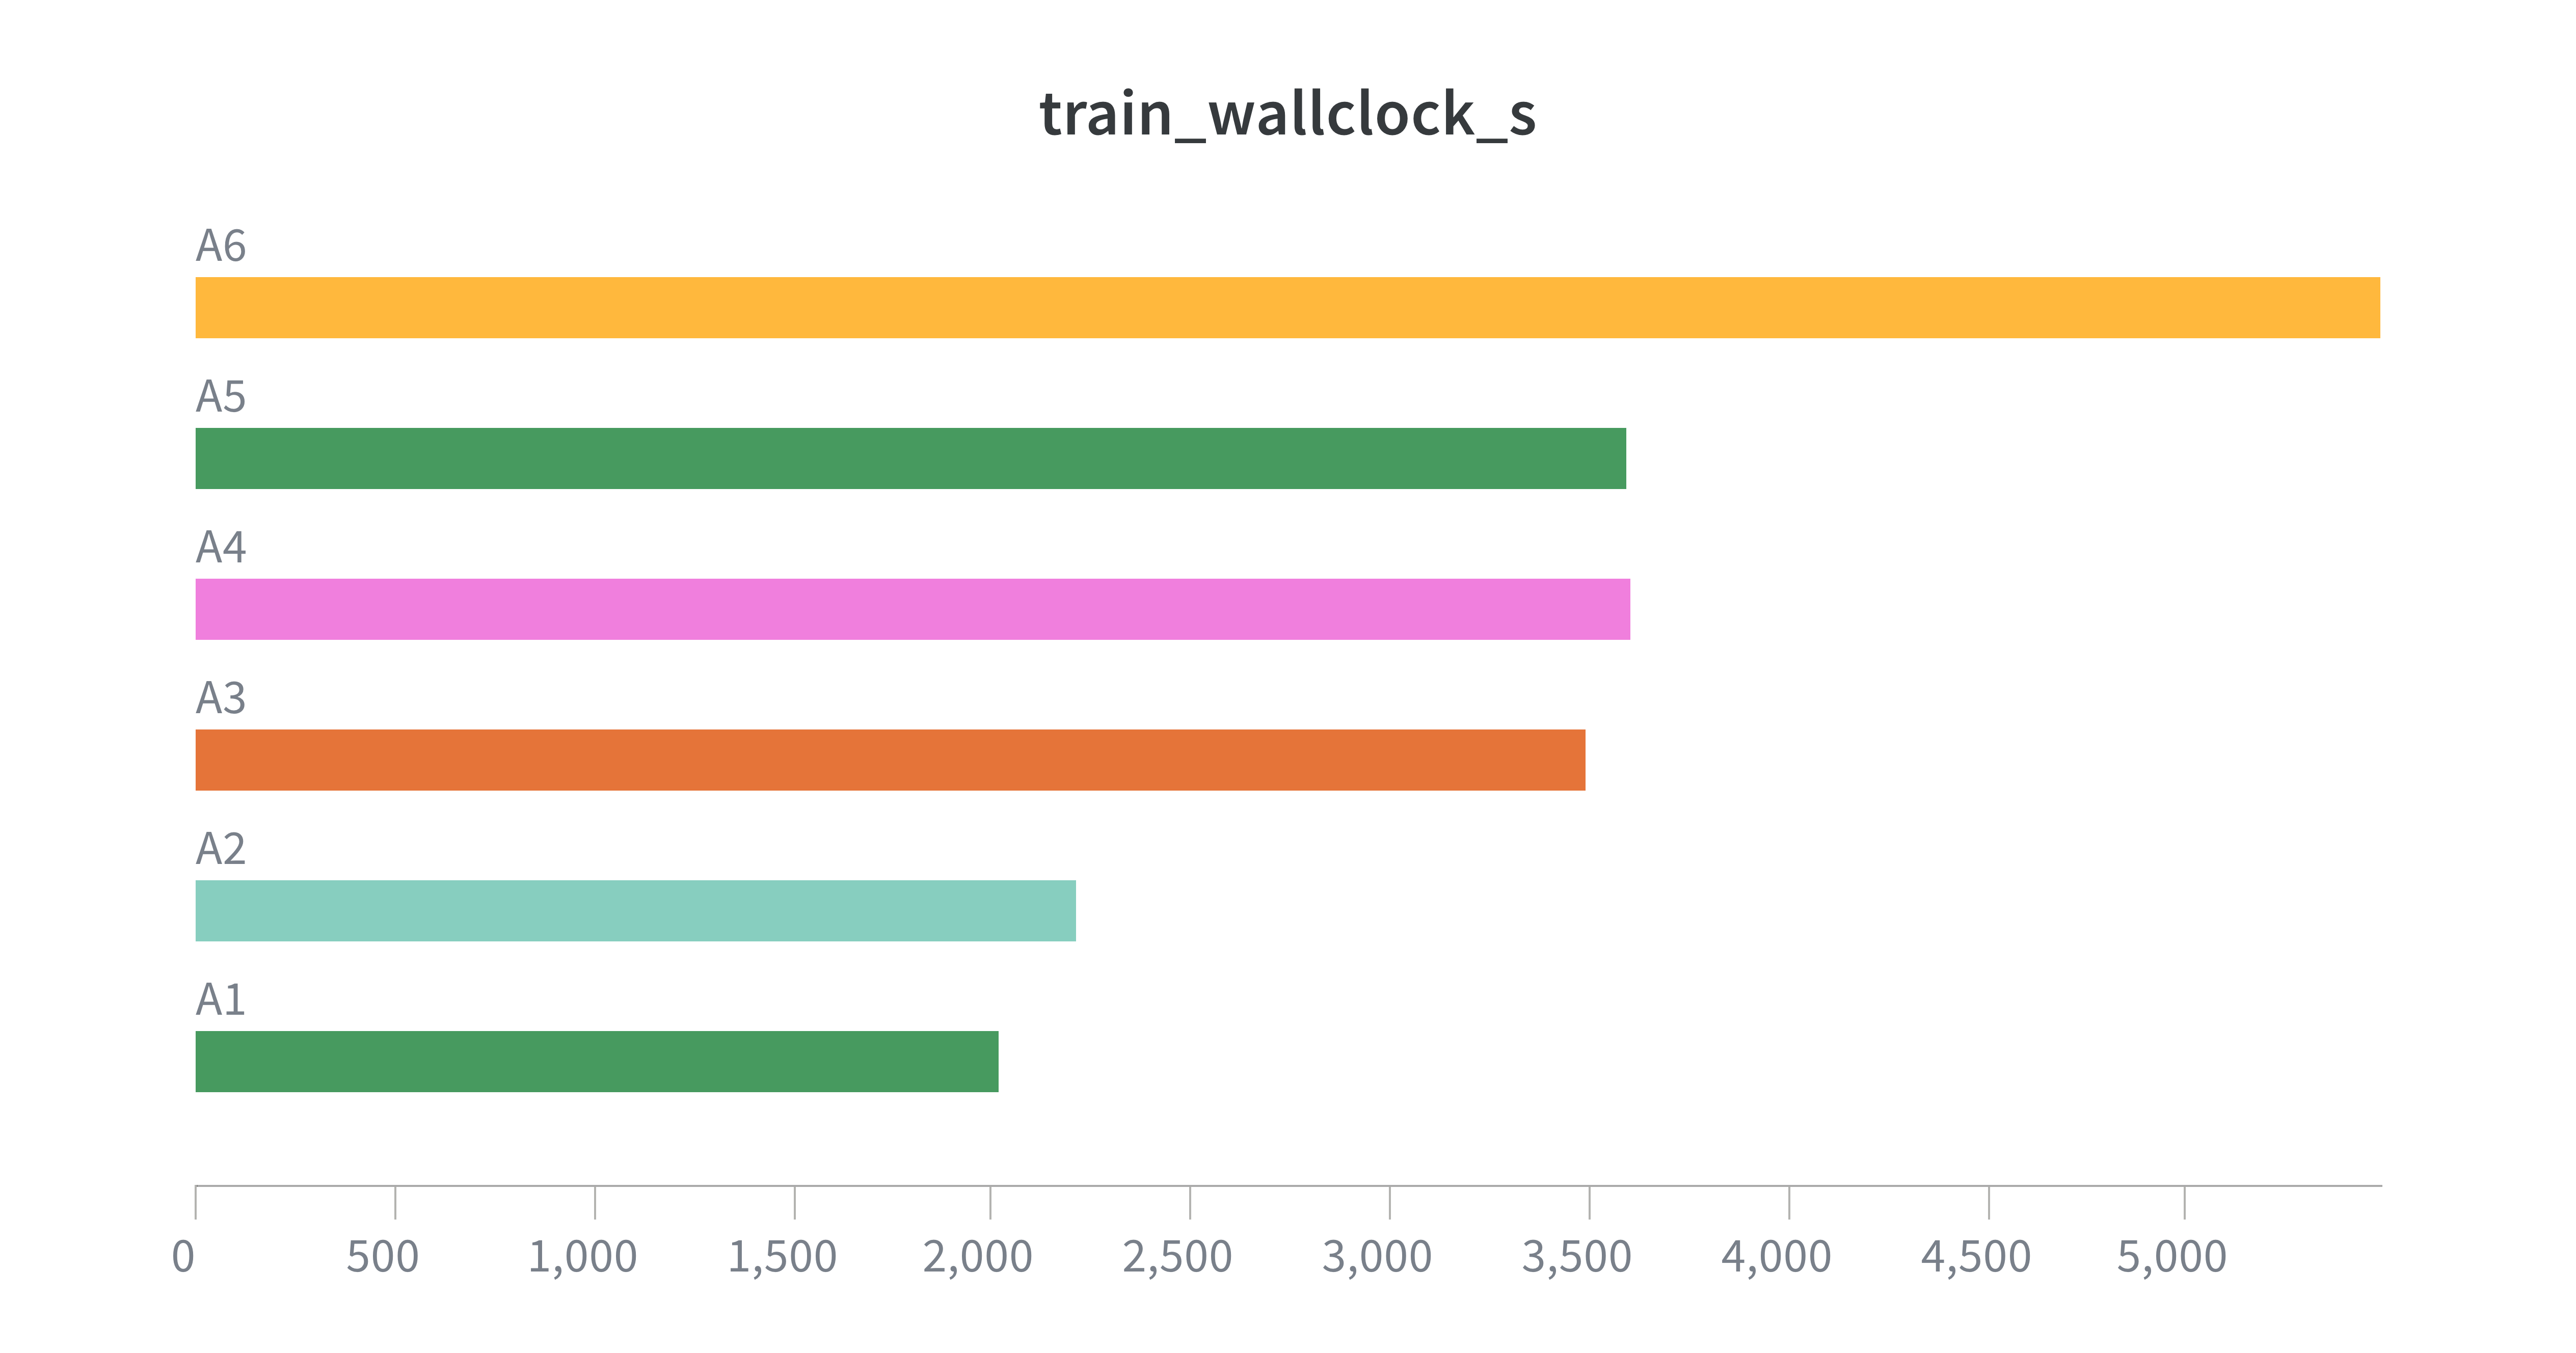
\includegraphics[width=0.49\textwidth]{assets/partA/wallclock_s.png}\hfill
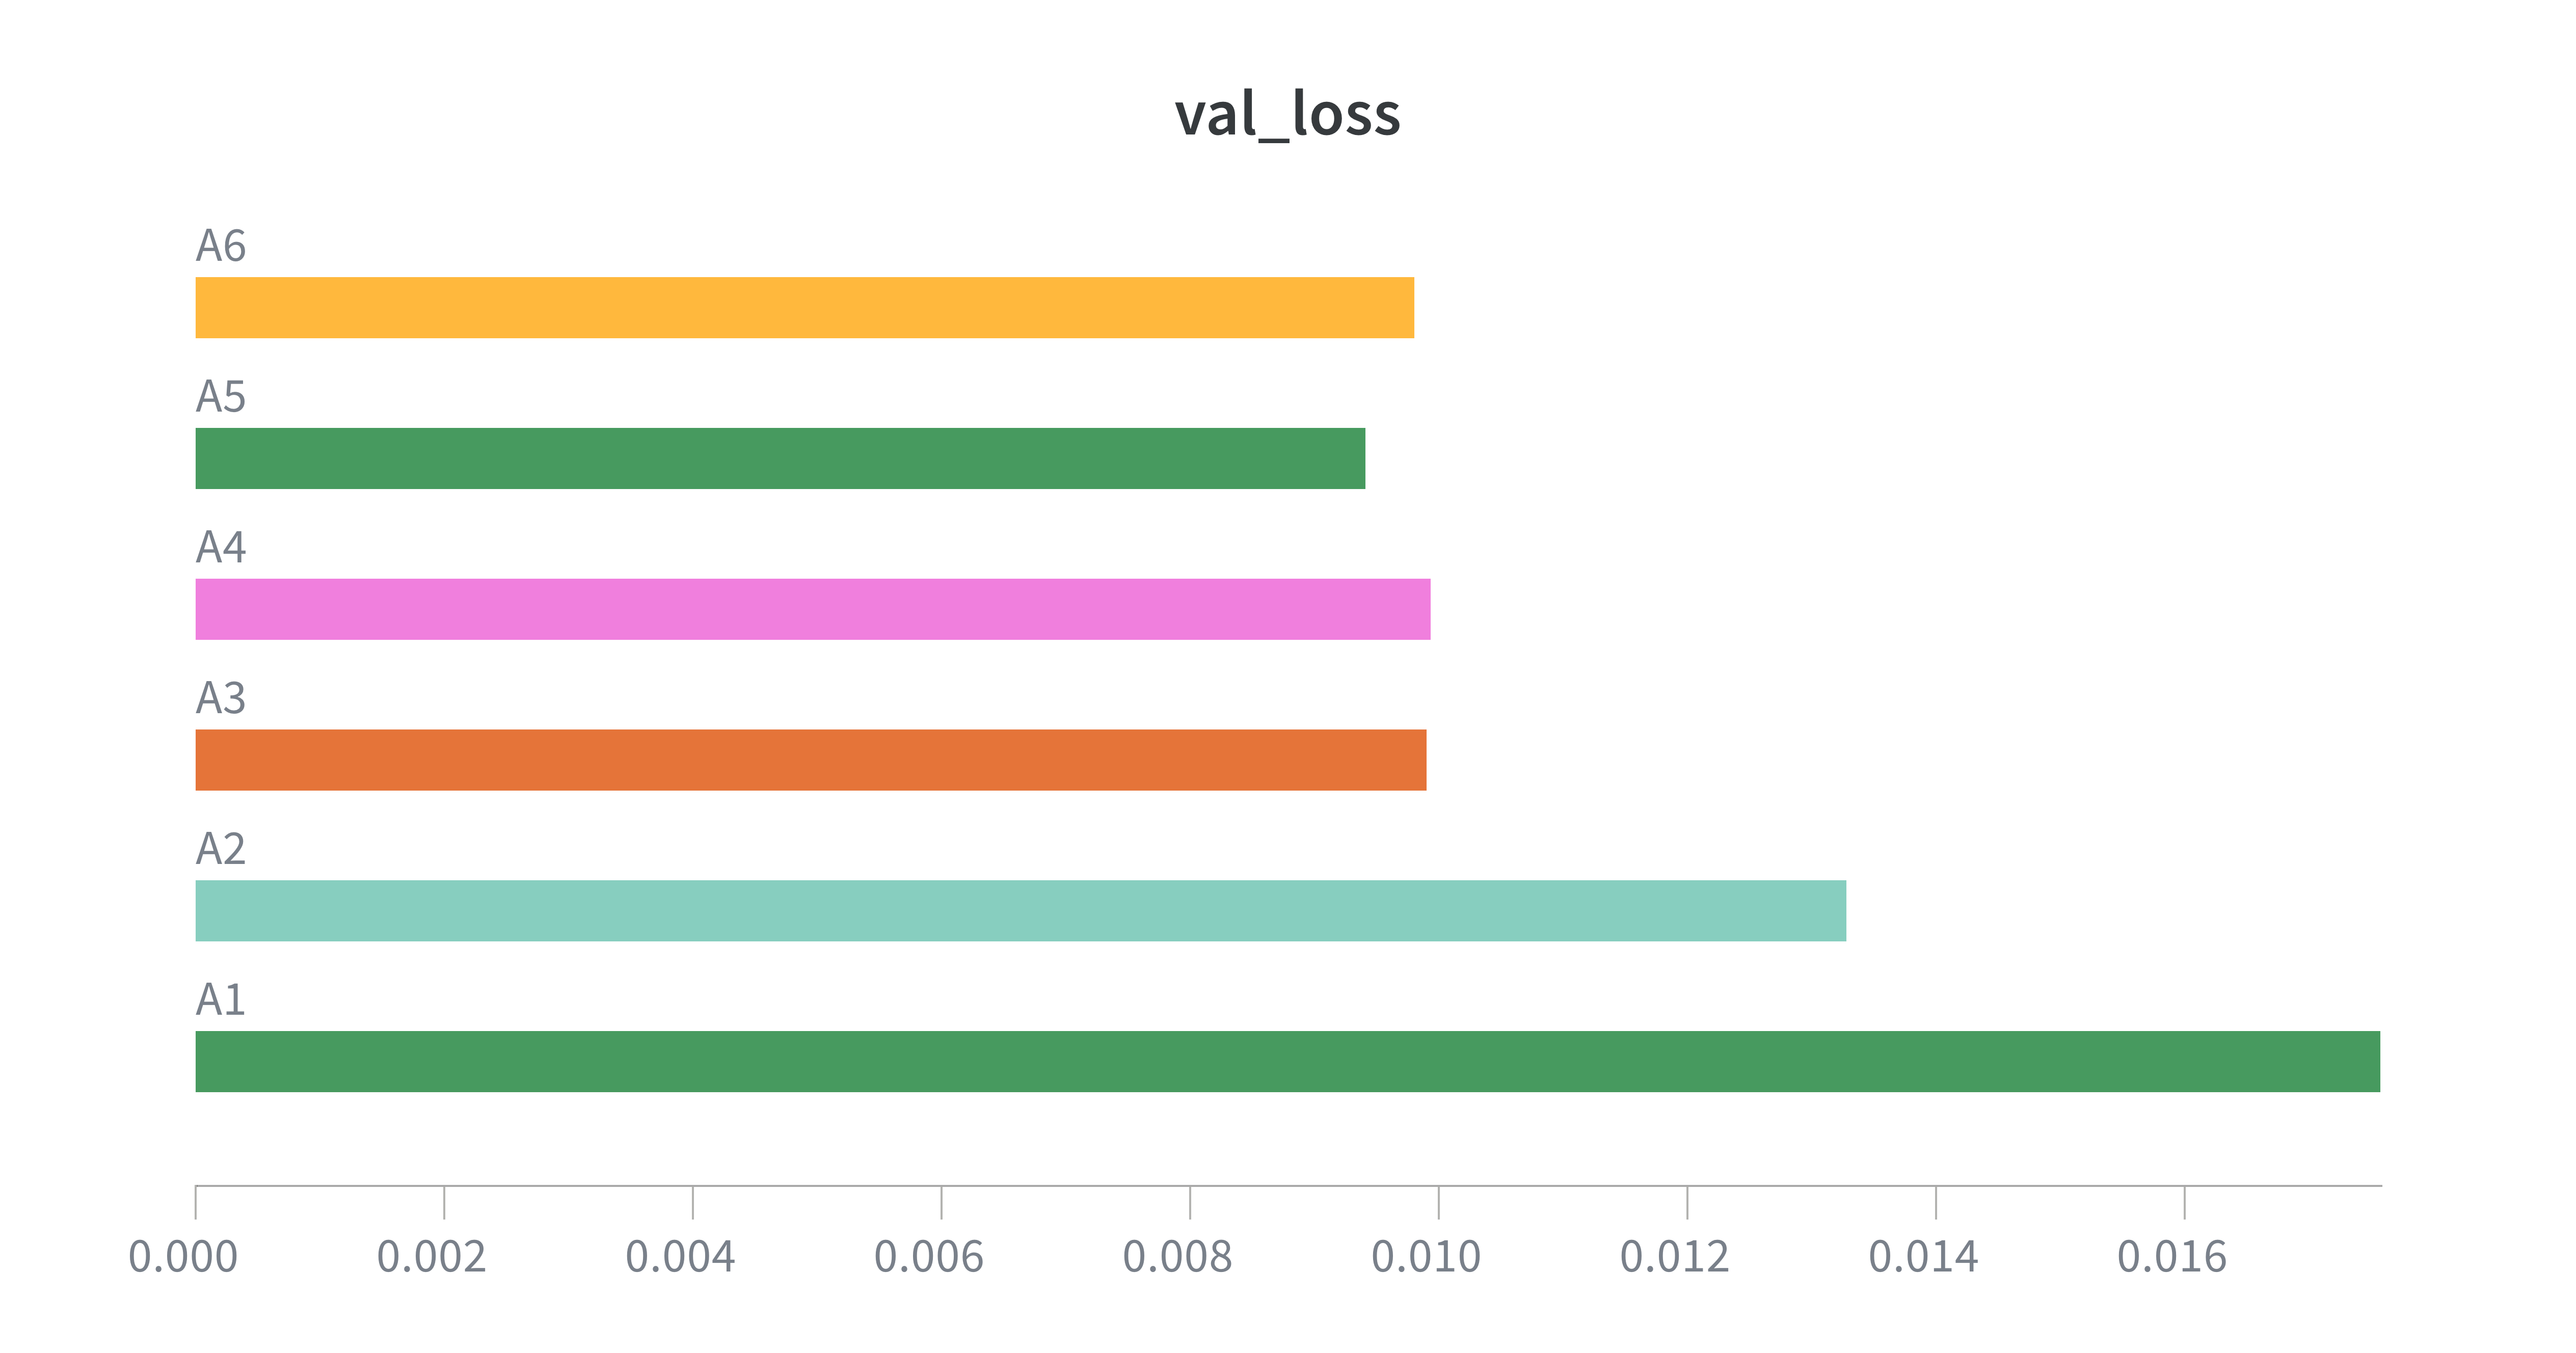
\includegraphics[width=0.49\textwidth]{assets/partA/val_loss.png}
\caption{Left: training time in seconds; the MLP layers (A3) add about 21 minutes and 4-bit QLoRA (A6) adds another 53\%. Right: validation loss, which keeps falling up to A5 even though F1 stops improving after A3.}
\label{fig:partA-cost}
\end{figure}

\subsection{B.1 span recovery: failure modes and their effect}\label{app:b1}
\textbf{Failure modes.} Three problems showed up while checking the outputs; the first two are fixed by rule 1, the third by rule 2.
\begin{itemize}
  \item \textbf{Brackets inside the value.} For \texttt{[52.2, -1.2]} $\to$ \texttt{[GEOCOORD]}, the brackets of the value were matched with the brackets of the tag, so the tag was not recognised. All 48 GEOCOORD spans and 56 passwords containing brackets were lost.
  \item \textbf{Several tags in one place.} For \texttt{Ab Male VAP451617O} $\to$ \texttt{[TITLE] [SEX] [IDCARD]}, only the first tag became a span.
  \item \textbf{A shared letter.} The \texttt{M} of \texttt{Marta} also appears in \texttt{[GIVENNAME1]}. The comparison matched it and split the tag in two, so the whole span was lost.
\end{itemize}
Problems that remain: two PII values next to each other can merge into one span (38 cases for A6, e.g.\ a phone number followed by an email); if the model changes nearby text, that text becomes part of the span; outputs that reorder the document cannot be lined up at all.

\textbf{Effect of these fixes on scores.} Scoring A6's test outputs with each version:

\begin{center}
\begin{tabular}{@{}lccc@{}}
\toprule
Span recovery & F1 (IoU $\ge$ 0.5) & Precision & Recall \\
\midrule
No fixes & 0.816 & \textbf{0.954} & 0.712 \\
+ shared-letter fix & 0.939 & 0.947 & 0.931 \\
+ one-character tags (final) & \textbf{0.954} & 0.950 & \textbf{0.958} \\
\bottomrule
\end{tabular}
\end{center}

\noindent Part A's validation F1 was computed before these fixes. That is why A6 has 0.815 on validation but 0.954 on test: with the unfixed code, test F1 is also 0.816 (A5: 0.809 vs.\ 0.807 on validation). So the model is not worse on validation; the old scorer lost about a quarter of the correct spans. All Part A runs were scored the same way, so they can still be compared with each other, but their F1 values are too low. Leak rate does not use spans, so Part A leak rates are correct.

\subsection{B.2 metric definitions and B.3 baseline details}\label{app:b2}
\begin{itemize}
  \item \textbf{Precision / recall / F1.} A predicted span is correct if it has the same label as a gold span and either the exact same boundaries (exact) or an overlap of IoU $\ge$ 0.5 (overlap). Micro F1 counts all spans together. Macro F1 averages the F1 of the 27 gold labels. Spans with invented labels count as wrong in micro F1 but are not added as extra labels to the macro average.
  \item \textbf{Leak rate.} Share of gold PII values that still appear in the output (ignoring case and extra spaces).
  \item \textbf{Over-masking rate.} Share of non-PII characters that were changed or removed.
  \item \textbf{Well-formed rate.} Share of outputs that are non-empty and between 0.5 and 1.5 times the input length.
\end{itemize}

\textbf{Note on leak rate.} Very short values are counted as leaked even when they were masked, because the same letters appear elsewhere in the text. For example, SEX \texttt{M} is found inside ``from'', and STATE \texttt{PA} inside other words. Of A6's 474 leaks, 349 are values of 1--2 characters like these. If we count only values the model did not mask, A6's leak rate is 0.8\% instead of 3.7\%. The table reports 3.7\%, as the assignment defines it.

\textbf{Baselines.}
\begin{itemize}
  \item \textbf{Regex.} Patterns for email, URL, IP, credit card, SSN, dates, times, postcodes, geo-coordinates, phone numbers, titles and sex. If two patterns overlap, the longer match wins. Every date is labelled DATE, because dates of birth (BOD) look exactly like other dates.
  \item \textbf{Presidio} with its default recognizers. Its labels are renamed to ours: PERSON$\to$GIVENNAME1, LOCATION$\to$CITY, DATE\_TIME$\to$DATE, PHONE\_NUMBER$\to$TEL, EMAIL\_ADDRESS$\to$EMAIL, IP\_ADDRESS$\to$IP, US\_SSN$\to$SOCIALNUMBER, US\_PASSPORT$\to$PASSPORT, US\_DRIVER\_LICENSE$\to$DRIVERLICENSE (each to the gold label it overlaps most often). Presidio has no separate time, date-of-birth or sex labels, so it can never get those right.
  \item \textbf{Qwen2.5-1.5B-Instruct without fine-tuning}, zero-shot and 5-shot. The 5 examples are the first 5 short rows ($\le$300 characters) of the training set.
\end{itemize}

\subsection{B.2 per-class results for A6}\label{app:perclass}
\begin{table}[h!]
\centering
\caption{A6 results for the 10 most frequent labels.}
\label{tab:partB-perclass}
\begin{tabular}{@{}lccccccc@{}}
\toprule
Class & Support & Exact P & Exact R & Exact F1 & IoU50 P & IoU50 R & IoU50 F1 \\
\midrule
TIME & 945 & 0.968 & 0.969 & 0.969 & 0.969 & 0.970 & 0.970 \\
USERNAME & 760 & 0.964 & 0.955 & 0.960 & 0.965 & 0.957 & 0.961 \\
SOCIALNUMBER & 668 & 0.961 & 0.969 & 0.965 & 0.961 & 0.969 & 0.965 \\
EMAIL & 662 & 0.973 & 0.980 & 0.977 & 0.978 & 0.985 & 0.981 \\
IDCARD & 651 & 0.948 & 0.943 & 0.945 & 0.951 & 0.946 & 0.948 \\
DRIVERLICENSE & 643 & 0.959 & 0.941 & 0.950 & 0.962 & 0.944 & 0.953 \\
LASTNAME1 & 623 & 0.900 & 0.891 & 0.895 & 0.903 & 0.894 & 0.898 \\
BOD & 553 & 0.964 & 0.973 & 0.968 & 0.975 & 0.984 & 0.979 \\
PASSPORT & 552 & 0.902 & 0.966 & 0.933 & 0.904 & 0.967 & 0.934 \\
SEX & 529 & 0.976 & 0.985 & 0.980 & 0.976 & 0.985 & 0.980 \\
\bottomrule
\end{tabular}
\end{table}

\noindent LASTNAME1 is the weakest label (F1 0.90), mostly because last names get called first names (16) or second last names (10). PASSPORT has lower precision (0.90) because other ID numbers get tagged as PASSPORT (driver licence 18, SSN 11, ID card 10).

\subsection{C.3(c) canary exposure numbers}\label{app:canary}
\begin{table}[h!]
\centering
\caption{Mean exposure by number of copies (maximum measurable: 13.29). Bold: lower exposure of V-raw and V-san.}
\label{tab:partC-canary}
\begin{tabular}{@{}lcccc@{}}
\toprule
Model & 1 copy & 4 copies & 16 copies & 64 copies \\
\midrule
Base  & 1.38 & 2.08 & 1.41 & 3.16 \\
V-raw & 13.29 & 13.29 & 13.29 & 13.29 \\
V-san & \textbf{2.47} & \textbf{3.45} & \textbf{1.28} & \textbf{1.27} \\
\bottomrule
\end{tabular}
\end{table}

% =====================================================
\section*{Honour Code}
\noindent\textit{``Even though I have taken help from the following students and LLMs in terms of discussing ideas and coding practices, all my code is written by me.''}

\vspace{0.5em}
\noindent \textbf{Students consulted:} None

\noindent \textbf{LLMs / tools used:}
Claude Code

\end{document}
